\subsection{Tree-based models}\label{sec:tree_based_models}

We also considered tree-based models as a meta-modelling approach. One advantage of these models is that they can handle categorical variables naturally, such as gender and product type. Moreover, they can capture non linear effects and interactions between variables. Other great advantages of tree-based models are their ability to perform feature selection and the fact that they are also easy to interpret by checking the tree structure.

%        \begin{itemize}
%            \item Quan, Zhiyu \& Gan, Guojun \& Valdez, Emiliano. (2018). Tree-based Models for Variable Annuity Valuation: Parameter Tuning and Empirical Analysis. SSRN Electronic Journal
%           	 \item Tree-based models can handle categorical variables naturally
%            \item Tree-based models can capture non linear effects and interactions between variables
 %           \item Tree-based models can perform feature selection
  %          \item Easy to interpret by checking the tree structure
   %     \end{itemize}



				
%To study such models we used primarily the work of quan2018treefollowing paper:
%Quan, Zhiyu \& Gan, Guojun \& Valdez, Emiliano. (2018). Tree-based Models for Variable Annuity Valuation: Parameter Tuning and Empirical Analysis. SSRN Electronic Journal.
%In this paper, the authors compare the performance of several different tree models in predicting the fair market value of VAs.

To study such models we used primarily~\cite{quan2018tree}, where the authors compare the performance of several different tree models in predicting the fair market value of VAs. As shown in Table~\ref{tab:tree}, we can see that generally, the Gradient boosting performed better. With that in mind, we focus on this method.

\begin{table}
\makebox[\textwidth][c]{
\begin{tabular}{cccccccc}
\toprule
Model & Gini & $R^2$ & CCC & ME & PE & MSE & MAE \\
\midrule
Regression tree (CART)      &  0.786    &  0.845     & 0.917    &  1.678   & -0.025   & 3278.578    & 31.421 \\
Bagged trees                & 0.842     &  0.918     & 0.954    &  2.213   & -0.033   & 1720.725    & 20.334 \\
Gradient boosting           & 0.836     &  0.942     & 0.969    &  1.311   & -0.019   & 1214.899    & 19.341 \\
Conditional inference trees & 0.824     &  0.869     & 0.930    &  0.905   & -0.013   & 2754.853    & 26.536 \\
Conditional random forests  & 0.836     &  0.892     & 0.940    &  1.596   & -0.024   & 2273.385    & 23.219 \\
Ordinary Kriging            & 0.815     &  0.857     & 0.912    & -0.812   &  0.012   & 3006.192    & 27.429 \\
GB2                         & 0.827     &  0.879     & 0.930    &  0.106   & -0.002   & 2554.246    & 27.772 \\
\bottomrule
\end{tabular}
}
\caption{Prediction accuracy of different models}\label{tab:tree}
\end{table}

%We can see that generally, the Gradient boosting performed better. With that in mind, let us look into this method more deeply:
%        \begin{itemize}
%            \item Quan, Zhiyu \& Gan, Guojun \& Valdez, Emiliano. (2018). Tree-based Models for Variable Annuity Valuation: Parameter Tuning and Empirical Analysis. SSRN Electronic Journal
%        \end{itemize}
%        \begin{figure}
% 			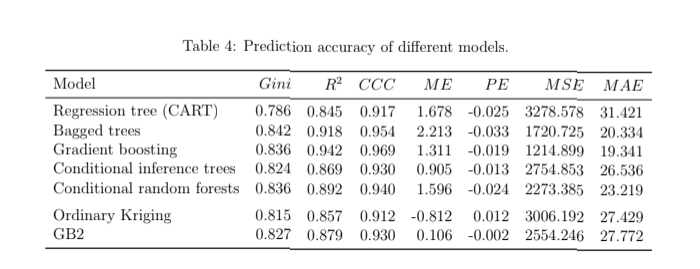
\includegraphics[width=1.0\linewidth]{pictures/emiliano_tree.png}
%   			\caption{Prediction accuracy of different models}
% 		\end{figure} 
        % inserir a imagem

%        \begin{itemize}
%			\setlength\itemsep{0,7em}
%            \item A gradient boosting regression tree is an ensemble model which grows trees by sequentially putting more weights on residuals of previous trees
 %           \item The final tree is given by:
  %          $$f_{B}(\mathbf{X})=\sum_{b=1}^{B} T_{b}\left(\mathbf{X} ; \Theta_{b}\right)$$
   %      	\item where $T_{b}\left(\mathbf{X} ; \Theta_{b}\right)$ are the regression trees. $B$ is the number of iterations or the number of additive trees. In each step $b,$ for $b=1, \ldots, B,$ we need to find the regression $\Theta_{b}$ based on
%the following optimization problem:
%
 %        	$$\hat{\Theta}_{b}=\underset{\Theta_{b}}{\arg \min } \sum_{i=1}^{N} L\left(y_{i}, f_{b-1}\left(\mathbf{X}_{i}\right)+T_{b}\left(\mathbf{X}_{i} ; \Theta_{b}\right)\right)$$
         	
  %      \end{itemize}

A gradient boosting regression tree is an ensemble model which grows trees by sequentially putting more weights on residuals of previous trees. The final tree is given by:    
$$f_{B}(\mathbf{X})=\sum_{b=1}^{B} T_{b}\left(\mathbf{X} ; \Theta_{b}\right)$$
where $T_{b}\left(\mathbf{X} ; \Theta_{b}\right)$ are the regression trees, and $B$ is the number of iterations or the number of additive trees. In each step $b,$ for $b=1, \ldots, B,$ we need to find the regression $\Theta_{b}$ based on the following optimization problem:
	$$\hat{\Theta}_{b}=\underset{\Theta_{b}}{\arg \min } \sum_{i=1}^{N} L\left(y_{i}, f_{b-1}\left(\mathbf{X}_{i}\right)+T_{b}\left(\mathbf{X}_{i} ; \Theta_{b}\right)\right)$$
%        \begin{itemize}
%        	\setlength\itemsep{0,7em}
%            \item GBM using 1000 trees and maximum depth = 3
%            \item training for 100 random sets of representatives VAs, each containing 340 contracts
%            \item The error measure are smaller for the overlapped grouped lasso model
%            \item The error measures vary a lot more for the GBM tree model then for the overlapped grouped lasso model, suggesting that the former is more robust to the selection of the representative contracts
%        \end{itemize}
Being that the gradient boosting regression tree was the best model for our case, we wanted to compare its performance against the overlapped group lasso model, which had very good results, as shown in Section~\ref{sec:linear_model}. Furthermore, we wished to test the robustness of each model to the set of representative contracts. In order to do so, we trained each model with 100 random sets of representative VAs, each containing 340 contracts. We used 100 trees and maximum depth of 3 for the GBM. 
%The results follow below:
As the tables~\ref{gbm_erros} and~\ref{lasso_erros} show, the error measures are smaller for the overlapped grouped lasso model. Additionally, the error measures vary a lot more for the GBM tree model then for the overlapped grouped lasso model, suggesting that the former is more robust to the selection of the representative contracts.

\begin{table}[ht]
\centering
\begin{tabular}{rrrrrr}
\toprule
 & $|$PE$|$ & R2 & $|$ME$|$ & MAE & MSE \\
\midrule
%Rep. VAs: 340 & 0.17 & 0.74 & 16.95 & 57.85 & 7542.90 \\
  %Rep. VAs: 680 & 0.04 & 0.73 & 3.90 & 57.43 & 7809.42 \\
  Min. & 0.00 & 0.87 & 0.00 & 28.46 & 2180.66 \\
  1st Qu. & 0.01 & 0.89 & 1.41 & 30.72 & 2517.63 \\
  Median & 0.03 & 0.90 & 2.66 & 31.63 & 2776.60 \\
  Mean & 0.03 & 0.90 & 2.80 & 31.91 & 2822.27 \\
  3rd Qu. & 0.04 & 0.91 & 3.82 & 33.00 & 3053.23 \\
  Max. & 0.10 & 0.92 & 9.37 & 36.60 & 3858.51 \\
\bottomrule
\end{tabular}
\caption{GBM Tree: Error measures for multiple sets of representatives contracts}
\label{gbm_erros}
\end{table}

\begin{table}[ht]
\centering
\begin{tabular}{rrrrrr}
\toprule
 & $|$PE$|$ & R2 & $|$ME$|$ & MAE & MSE \\
\midrule
%Rep. VAs: 340 & 0.01 & 0.95 & 0.87 & 23.29 & 1377.79 \\
 %Rep. VAs: 680 & 0.01 & 0.96 & 1.16 & 20.89 & 1104.23 \\
  Min. & 0.00 & 0.93 & 0.08 & 18.59 & 810.84 \\
  1st Qu. & 0.00 & 0.96 & 0.40 & 20.79 & 1074.65 \\
  Median & 0.01 & 0.96 & 1.09 & 21.28 & 1163.91 \\
  Mean & 0.01 & 0.96 & 1.31 & 21.33 & 1182.15 \\
  3rd Qu. & 0.02 & 0.96 & 1.82 & 21.88 & 1248.26 \\
  Max. & 0.05 & 0.97 & 4.79 & 23.70 & 1911.56 \\
\bottomrule
\end{tabular}
\caption{Overlapped Group Lasso: Error measures for multiple sets of representatives contracts}
\label{lasso_erros}
\end{table}	

